\documentclass[11pt]{article}

% Change "review" to "final" to generate the final (sometimes called camera-ready) version.
% Change to "preprint" to generate a non-anonymous version with page numbers.
\usepackage[review]{acl}

% Standard package includes
\usepackage{times}
\usepackage{latexsym}

% For proper rendering and hyphenation of words containing Latin characters (including in bib files)
\usepackage[T1]{fontenc}

% This assumes your files are encoded as UTF8
\usepackage[utf8]{inputenc}

% This is not strictly necessary, and may be commented out,
% but it will improve the layout of the manuscript,
% and will typically save some space.
\usepackage{microtype}

% This is also not strictly necessary, and may be commented out.
% However, it will improve the aesthetics of text in
% the typewriter font.
\usepackage{inconsolata}

% Including images in your LaTeX document requires adding
% additional package(s)
\usepackage{graphicx}
\usepackage{url}

\usepackage{float}

\title{Deep Learning Midterm Project Report}

\author{[Your Name] \\
  New York University \\
  ECE-GY 7123 Deep Learning \\
  \texttt{[your email]}}

\begin{document}
\maketitle

\begin{abstract}
This report presents our approach to a deep learning task using modern neural
network methods. We focus on building a competitive model under practical
training-time constraints, compare multiple configurations, and summarize the
design and optimization choices that contributed most to performance.
\end{abstract}

\section{Introduction}

This project focuses on solving a deep learning task using modern neural network
approaches. The goal is to build a model that achieves strong performance on
the given dataset while exploring different architectural and training choices.

Due to the computational cost of training, we emphasize iterative
experimentation and practical improvements over exhaustive search. We evaluate
different configurations and analyze what contributes most to performance.

\footnote{Code: \url{https://github.com/shanpig/dl-kaggle-midterm}. We used GPT
and Cursor for debugging and implementation assistance.}

\footnote{Model weights: [ADD YOUR LINK HERE]}

\section{Dataset}

The dataset utilized in this study comprises paired natural language descriptions and Scalable Vector Graphics (SVG) code. The data is partitioned into a training set of 50,000 records (\texttt{train.csv}), which includes a unique identifier (\texttt{id}), a natural language prompt (\texttt{prompt}), and the ground-truth SVG code (\texttt{svg}). The evaluation set (\texttt{test.csv}) contains 1,000 records featuring only the identifier and prompt, tasking the model with generating the missing SVG format. To ensure robust training within the strict context window limitations of Large Language Models (LLMs), we validated the train-test distributional alignment and applied a deterministic preprocessing pipeline to structurally optimize the data without relying on synthetic augmentation.
\subsection{Dataset Alignment}
We verified consistency between the training and testing sets to prevent out-of-distribution evaluation. Textual prompts exhibit highly consistent lengths—averaging 19.79 and 20.14 words for the train and test sets, respectively—and share core vocabulary (e.g., ``black'', ``white'', ``icon'').

\begin{figure}[htbp]
    \centering
    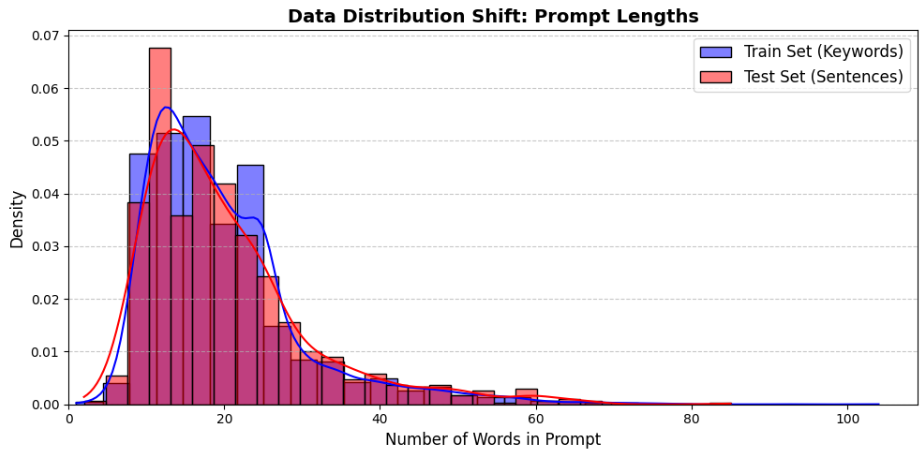
\includegraphics[width=0.48\textwidth]{TrainVsTest-2.png}
    \caption{Comparative analysis of textual distributions between the training and testing datasets.}
    \label{fig:train_vs_test-1}
\end{figure}

Structural visual complexity also aligns closely: the training set averages 2.8 XML tags per image, matching the NLP-predicted expectation of 2.87 tags for the test set.

\begin{figure}[htbp]
    \centering
    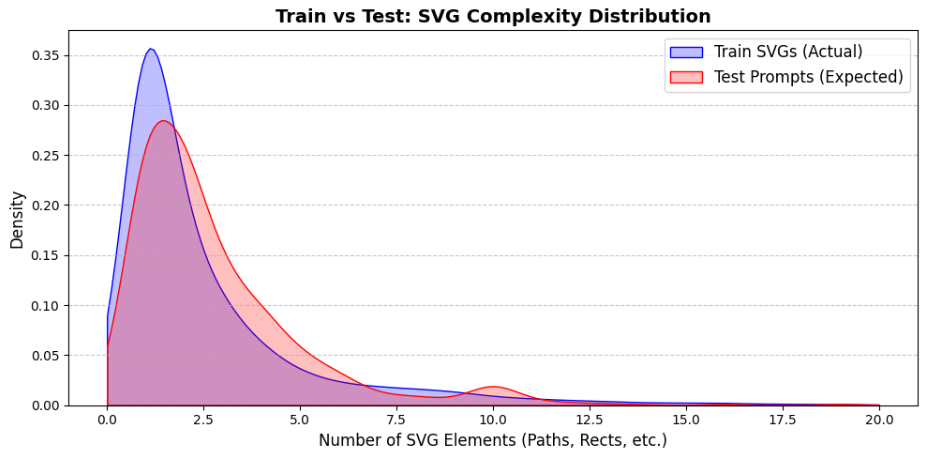
\includegraphics[width=0.48\textwidth]{TrainVsTest-1.png}
    \caption{Comparative analysis of structural distributions between the training and testing datasets.}
    \label{fig:train_vs_test-2}
\end{figure}

\subsection{Preprocessing and Optimization Pipeline}
Raw SVGs contain redundant metadata, arbitrary spatial dimensions, and high numerical precision that consume excessive tokens. To maximize semantic density while strictly constraining sequences to 8,000 characters and 256 path elements, we standardized 20,000 target samples through the following pipeline:

\begin{itemize}
    \item \textbf{Dimensional Standardization:} All canvases are mathematically scaled to a uniform $256 \times 256$ coordinate system. The algorithm extracts the original \texttt{viewBox} and proportionally updates all spatial attributes (e.g., \texttt{cx}, \texttt{width}, \texttt{d}) and complex transformation matrices (\texttt{translate}, \texttt{rotate}), establishing a fixed spatial representation for the model.
    \item \textbf{Tag Sanitization:} To prevent hallucination of proprietary metadata, we enforce a strict whitelist of 13 geometric tags (e.g., \texttt{path}, \texttt{rect}, \texttt{g}, \texttt{circle}). Unsupported elements and redundant styling attributes (such as \texttt{filling} and default opacities) are completely discarded.
\end{itemize}

\begin{figure}[H]
    \centering
    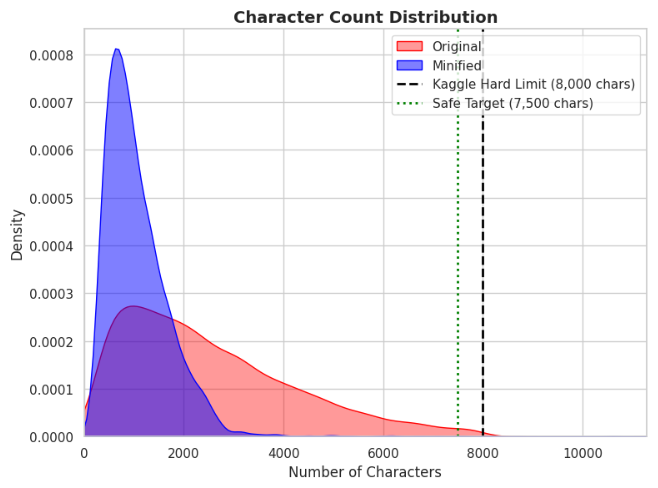
\includegraphics[width=0.48\textwidth]{Minimization-1.png}
    \caption{Structural representation of the training SVGs in characters before and after minimization and preprocessing pipeline.}
    \label{fig:minimization-2}
\end{figure}

\begin{itemize}
    \item \textbf{Token Minification:} Numerical coordinates are aggressively rounded to reduce sequence length, removing decimals for whole numbers and limiting floats to one decimal place (e.g., 12.5). XML headers, newlines, and extraneous whitespace are stripped entirely, flattening the hierarchical tree into a dense, continuous string.
    \item \textbf{Formatting:} Tabular features are standardized (renamed to \texttt{prompt} and \texttt{svg}), stripped of invalid XMLs, and formatted for direct compatibility with Hugging Face training libraries.
\end{itemize}

\begin{figure}[H]
    \centering
    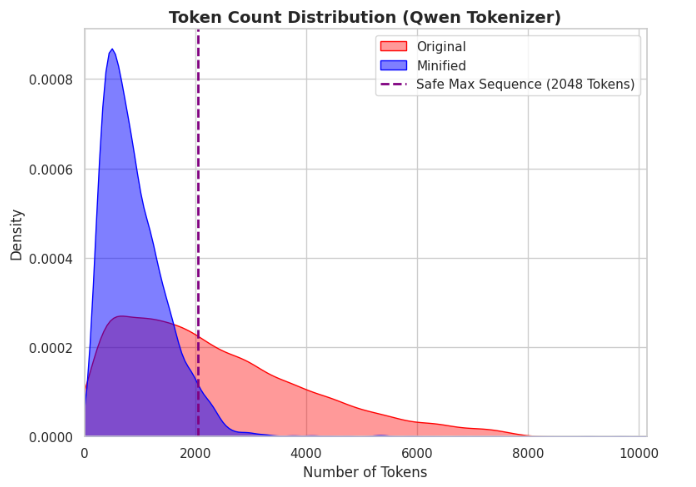
\includegraphics[width=0.48\textwidth]{Minimization-2.png}
    \caption{Structural representation of the training SVGs in tokens before and after minimization and preprocessing pipeline.}
    \label{fig:minimization-1}
\end{figure}

Ultimately, these interconnected preprocessing steps heavily constrain the problem space, significantly reducing token overhead while maintaining visual fidelity.
This structurally sound, token-optimized data allows the model to efficiently learn the highly complex mapping between natural language descriptions and valid geometric code without the need for additional data augmentation.

\begin{figure}[htbp]
    \centering
    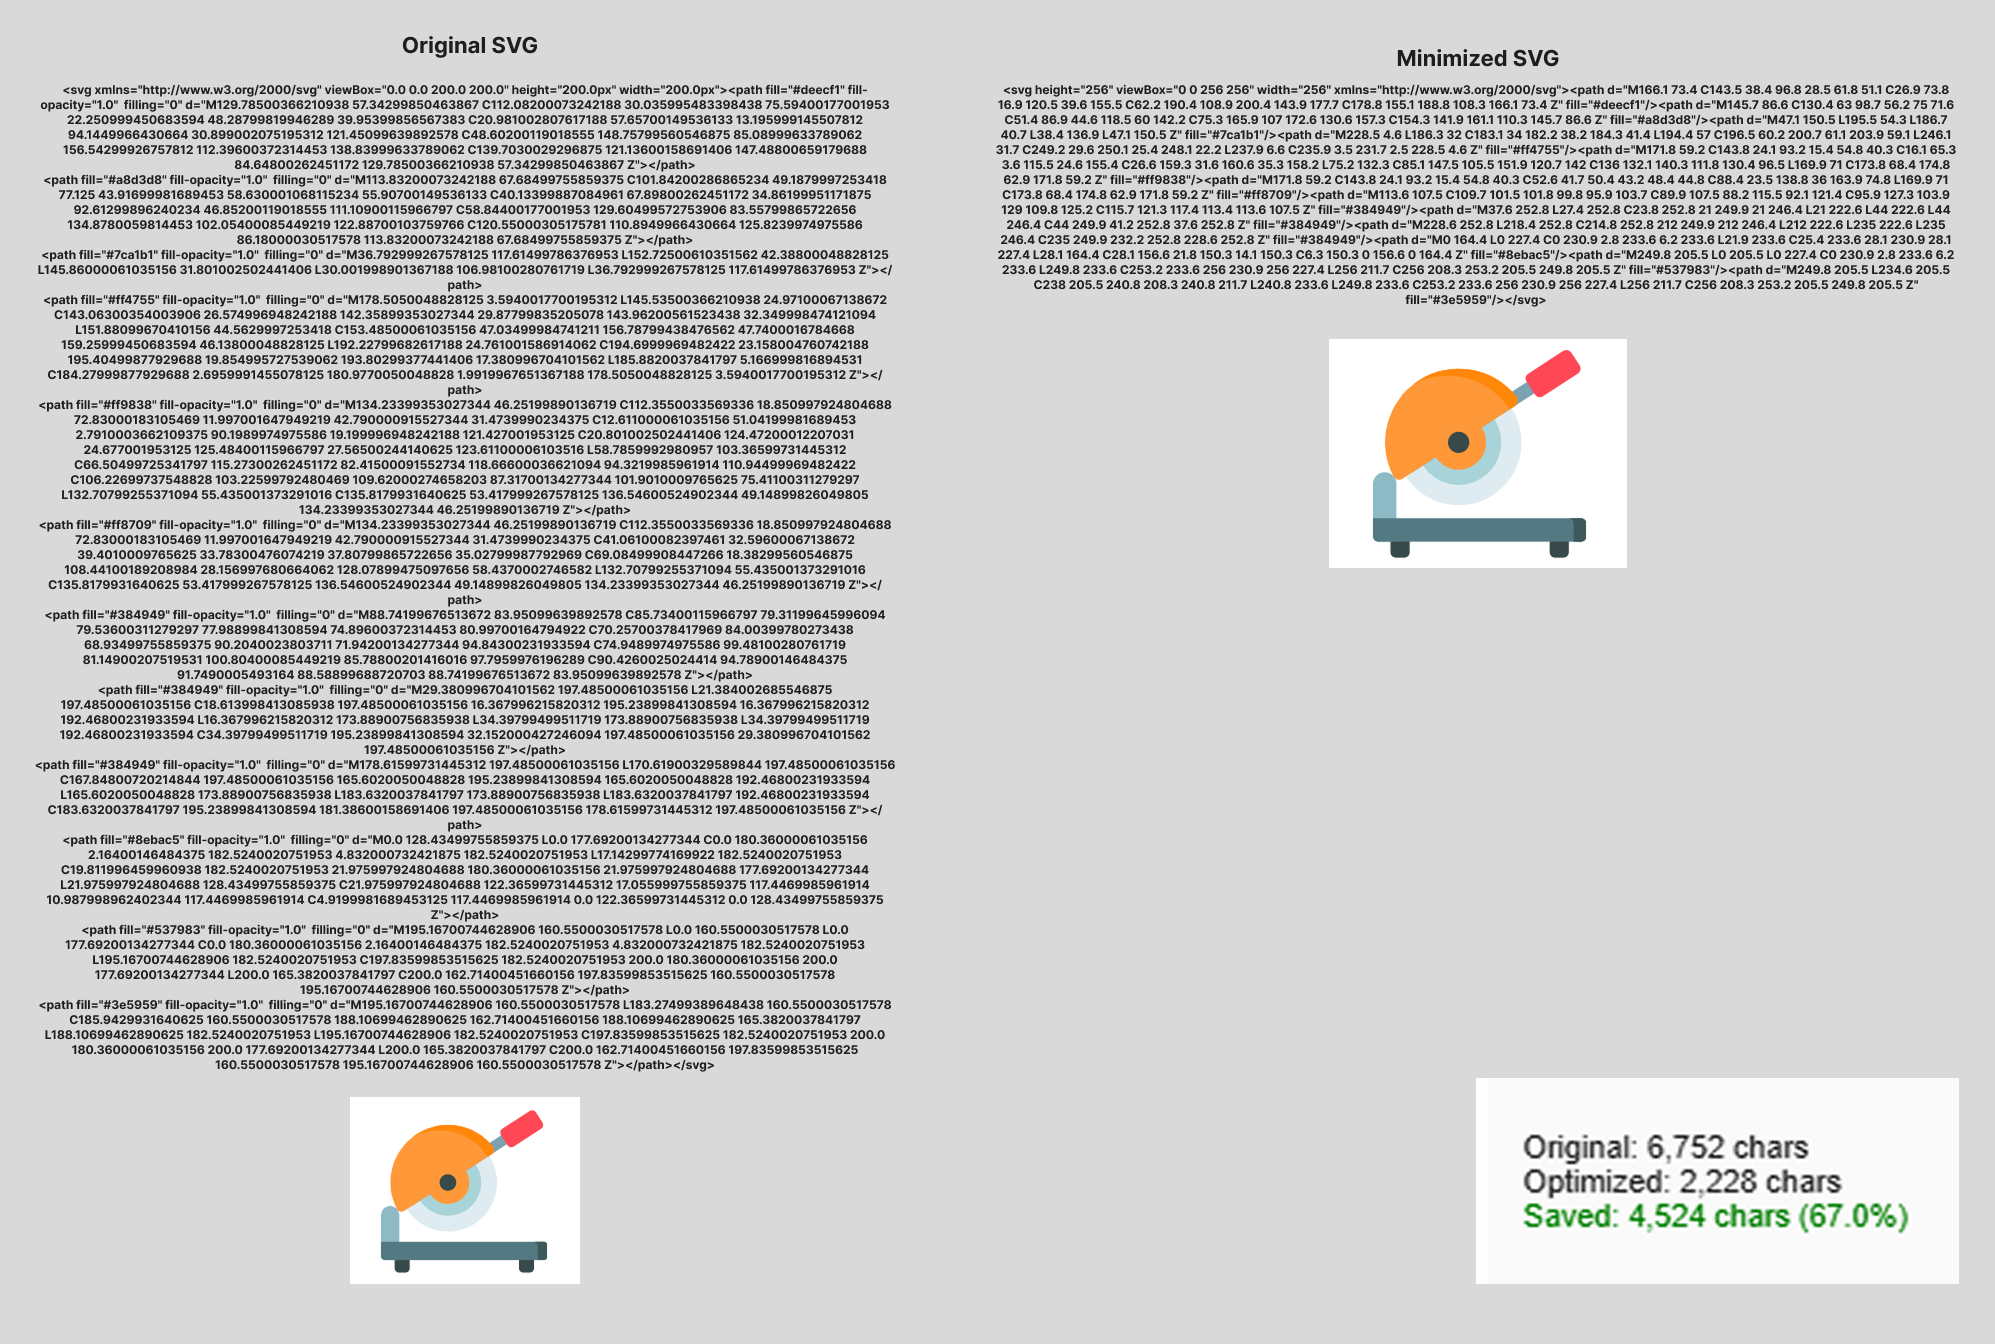
\includegraphics[width=0.48\textwidth]{MinimizationExample.png}
    \caption{Visual and code representation of an SVG before and after minimization and preprocessing pipeline.}
    \label{fig:minimization-3}
\end{figure}

\section{Model Description}

We implemented a deep learning model to address the task, starting from a
baseline architecture and iteratively improving it.

Our approach focuses on leveraging neural network architectures that can
effectively capture patterns in the data. We experimented with different
configurations to balance model capacity and training efficiency.

The model design was guided by the need for strong performance while keeping
training time manageable.

\section{Experimentation}

We conducted multiple experiments to improve model performance through
iterative refinement.

\textbf{Hyperparameters:}
\begin{itemize}
    \item Learning rate: [fill if known, e.g., 1e-3, 1e-4]
    \item Batch size: [e.g., 16, 32]
    \item Number of epochs: [range or estimate]
\end{itemize}

\textbf{Experimented Variations:}
\begin{itemize}
    \item Baseline model configuration
    \item Adjustments to model architecture
    \item Different training settings (learning rate, batch size)
\end{itemize}

Due to long training cycles, we focused on testing a limited number of
meaningful configurations rather than performing an exhaustive search. We
prioritized changes that were most likely to impact performance based on
intuition and prior experience.

\section{Results}

\begin{table}[t]
    \centering
    \begin{tabular}{lc}
        \hline
        Model & Score \\
        \hline
        Baseline & [XX.X] \\
        Final Model & [XX.X] \\
        \hline
    \end{tabular}
    \caption{Comparison between the baseline and final model performance.}
\end{table}

The final model achieved improved performance compared to the baseline. We
observed that tuning hyperparameters, particularly learning rate and model
configuration, had a noticeable impact on results.

In some cases, increasing model complexity did not yield proportional
improvements, indicating diminishing returns.

\section{Conclusion}

In this project, we explored different modeling approaches and training
strategies to improve performance on the task.

We found that careful tuning of hyperparameters and iterative experimentation
were key to achieving better results. However, training time posed a
significant constraint, limiting the number of experiments that could be
conducted.

Some approaches did not lead to improvements, highlighting the importance of
targeted experimentation rather than blindly increasing complexity.

In future work, we would implement better experiment tracking and explore more
efficient training methods to allow broader exploration of the design space.

\end{document}
